% !TeX program = lualatex
\documentclass[12pt,a4paper]{report}

% --------------------- PACKAGES ---------------------
\usepackage{fontspec}             % Custom font
\usepackage{pdfpages}             % Atach PDFs
\usepackage{graphicx}             % Images
\usepackage{amsmath,amssymb}      % Math
\usepackage{caption}              % Figure/table captions
\usepackage{subcaption}           % Subfigures
\usepackage{geometry}             % Margins
\usepackage{fancyhdr}             % Headers/footers
\usepackage{tocloft}              % ToC/List formatting
\usepackage[acronym,nonumberlist]{glossaries} % Acronyms
\usepackage[hidelinks]{hyperref}  % Hyperlinks
\usepackage{titlesec}             % Section title styling
\usepackage{listings}             % Source code
\usepackage{chngcntr}             % Counter tweaks
\usepackage{tabularx}             % Tables
\usepackage{tikz}                 % Graphs
\usepackage{pgfplots}             % Plots
\pgfplotsset{compat=1.18}         % Or latest version supported by Overleaf
\usepgfplotslibrary{groupplots}   % Required for group plots
\usepackage{booktabs}             % Better tables
\usepackage{setspace}             % For line spacing
\usepackage{csquotes}             % For biblatex + babel
\usepackage[romanian]{babel}      % For translating bibliography
\usepackage[backend=biber, style=ieee, language=auto]{biblatex} % Bibliography
\addbibresource{references.bib}

% --------------------- FORMAT ---------------------
\setmainfont{UTSans-Regular.otf}[
    Path = Fonts/,
    BoldFont = UTSans-Bold.otf,
    ItalicFont = UTSans-Regular.otf,
    ItalicFeatures={FakeSlant=0.2},
]
\geometry{top=2.5cm, bottom=2cm, left=2.5cm, right=1.5cm}
\setlength{\parindent}{1.25cm}
\linespread{1.2}
\makeglossaries%

% ------- STYLES
\titleformat{\chapter}
    {\normalfont\fontsize{18}{16}\bfseries\selectfont
    \raggedleft\rightskip=0.3cm}
    {\thechapter}{16pt}{\MakeUppercase}
\titlespacing{\chapter}{0pt}{18pt}{8pt}

\titleformat{\section}
    {\normalfont\fontsize{14}{16}\bfseries\selectfont}
    {\thesection}{16pt}{\MakeUppercase}
\titlespacing{\section}{0pt}{18pt}{0pt}

\titleformat{\subsection}
    {\normalfont\fontsize{12}{16}\bfseries\selectfont}
    {\thesubsection}{16pt}{}
\titlespacing{\subsection}{1.25cm}{10pt}{0pt}

\renewcommand{\normalsize}{\fontsize{12}{16}\selectfont}

% ------- HEADER & FOOTER
\pagestyle{fancy}
    \setlength{\headheight}{18pt}
    \setlength{\footskip}{70pt}
    \fancyhf{}
    \fancyhead[L]{
    \ifodd\value{page}{\projecttitle}
    \else\makebox[0pt][l]{\parbox[b]{\headwidth}{\raggedleft{\studentname}}}
    \fi}
    \fancyfoot[C]{\raisebox{15mm}{\thepage}}

\fancypagestyle{plain}{
    \fancyhf{}
    \fancyhead[L]{
    \ifodd\value{page}{\projecttitle}
    \else\makebox[0pt][l]{\parbox[b]{\headwidth}{\raggedleft{\studentname}}}
    \fi}
    \fancyfoot[C]{\raisebox{15mm}{\thepage}}
}

\fancypagestyle{plainfooter}{
  \fancyhf{}
  \renewcommand{\headrulewidth}{0pt}\setlength{\footskip}{70pt}
  \fancyfoot[C]{\raisebox{15mm}{\thepage}}
}

% --------------------- FIGURE, TABLE & CODE STYLES -----------------

% ------- TABLE OF CONTENTS
\renewcommand{\cftchapdotsep}{\cftdotsep}
\setlength{\cftchapnumwidth}{3em}
\renewcommand{\cftchapleader}{\cftdotfill{\cftchapdotsep}}
\AtBeginDocument{\renewcommand\contentsname{}}

% ------- BIBLIOGRAPHY
\defbibheading{bibliography}[\refname]{\chapter{Bibliografie}}
\renewcommand*{\bibfont}{\small}

% ------- FIGURES
\captionsetup{
    font=small,
    labelfont=bf,
    labelsep=period
}

\AtBeginDocument{
    \renewcommand{\figurename}{Figura}
    \counterwithout{figure}{chapter}
    \renewcommand{\listfigurename}{}
    \renewcommand{\cftfigpresnum}{Figura~}
    \renewcommand{\cftfigaftersnum}{.} 
    \settowidth{\cftfignumwidth}{Figură 100.} 
}

% For removing extra space in list of figures
% \makeatletter
% \def\@chapter[#1]#2{
%   \ifnum\c@secnumdepth>\m@ne%
%     \refstepcounter{chapter}
%     \typeout{\@chapapp\space\thechapter.}
%     \addcontentsline{toc}{chapter}{\protect\numberline{\thechapter}#1}
%   \else \addcontentsline{toc}{chapter}{#1} \fi
%   \chaptermark{#1}
%   \addtocontents{lot}{\protect\addvspace{10\p@}}
%   \if@twocolumn\@topnewpage[\@makechapterhead{#2}] 
%   \else \@makechapterhead{#2} \@afterheading\fi}
% \makeatother

% ------- TABLES
\captionsetup[table]{
    justification=raggedleft,
    singlelinecheck=false
}

\AtBeginDocument{
    \counterwithout{table}{chapter}
    \renewcommand{\listtablename}{}
    \renewcommand{\cfttabpresnum}{Tabelul~}
    \renewcommand{\cfttabaftersnum}{.}
    \settowidth{\cfttabnumwidth}{Tabelul 100.}
    \renewcommand{\tablename}{Tabelul}
}

\newcolumntype{L}[1]{>{\raggedright\arraybackslash}p{#1}}
\newcolumntype{C}[1]{>{\centering\arraybackslash}m{#1}}

% For removing extra space in list of tables
% \makeatletter
% \def\@chapter[#1]#2{
%   \ifnum\c@secnumdepth>\m@ne
%     \refstepcounter{chapter}
%     \typeout{\@chapapp\space\thechapter.}
%     \addcontentsline{toc}{chapter}{\protect\numberline{\thechapter}#1}
%   \else \addcontentsline{toc}{chapter}{#1} \fi
%   \chaptermark{#1}
%   \addtocontents{lot}{\protect\addvspace{0pt}}
%   \if@twocolumn\@topnewpage[\@makechapterhead{#2}]
%   \else\@makechapterhead{#2}\@afterheading\fi}
% \makeatother

% ------- SOURCE CODE
\lstset{
  basicstyle=\fontspec{Courier New}\fontsize{12}{9.6}\selectfont,
  numbers=left,
  numberstyle=\scriptsize,
  breaklines=true,
  captionpos=b,
  frame=none,
  showstringspaces=false,
  xleftmargin=0.6cm,
}

% --------------------- ACRONYMS ---------------------
% ------- ADD ALL ACRONYMS HERE - REFERENCE THEM IN TEXT WITH \gls{name}
\newacronym{aicors}{AICoRS}{Artificial Intelligence-enabled Hardware Cosmic Radiation Sensor for Space Applications}
\newacronym{bga}{BGA}{Ball Grid Array}
\newacronym{bram}{BRAM}{Block Random-Access Memory}
\newacronym{can}{CAN}{Controller Area Network}
\newacronym{cmos}{CMOS}{Complementary Metal–Oxide–Semiconductor}


% --------------------- DOCUMENT ---------------------
% ------- UPDATE HERE WITH CORRESPONDING VALUES - NAME & TITLE
\newcommand{\studentname}{Nume Prenume}
\newcommand{\projecttitle}{Titlul lucrării}

\begin{document}

% ------- THIS DOCUMENT IS MADE SEPARATELY AND ADDED HERE
% ------- NO NEED TO MODIFY HERE - JUST UNCOMMENT

\includepdf[pages=-, pagecommand={\thispagestyle{plainfooter}}] {Anexe/Prima pagina.pdf}

% ------- THE FOLLOWING PAGES ARE AUTOMATED - NO NEED TO MODIFY
\chapter*{Cuprins}
\vspace{-8em}
\tableofcontents
\newpage

\chapter*{Lista figurilor și tabelelor}
\addcontentsline{toc}{chapter}{Lista figurilor și tabelelor}

\section*{Figuri}
\vspace{-6em}
\listoffigures
\newpage

\section*{Tabele}
\vspace{-6em}
\listoftables
\newpage

\begingroup
\small
\setstretch{0.8}
\printglossary[type=acronym, style=list, nonumberlist, nogroupskip,title=Listă de acronime]
\endgroup
\addcontentsline{toc}{chapter}{Listă de acronime}
\newpage

% ------- THIS IS WHERE THE MAIN CONTENT GOES - EDIT HERE
\chapter{Introducere}
\section{Context și motivație}
Odată cu avansul tehnologic accelerat al umanității și evoluția domeniilor precum electronica, fizica și știința materialelor, aplicațiile aeronautice și spațiale capătă o importanță din ce în ce mai mare. Explorarea acestor medii extreme crește substanțial riscurile cauzate de radiația cosmică intensă prezentă în afara atmosferei. Din acest motiv, există un interes crescut în reducerea acestor pericole, prin studierea efectelor radiației ionizante, îmbunătățirea tehnologiilor de fabricare și protejare a componentelor, precum și detectarea și măsurarea nivelului de radiație. \textbf{Exemple de citații:} \cite{radiation_sensor_types} \cite{gaseours_detectors}. \textbf{Exemple de acronime:} \gls{aicors}, \gls{bga}, \gls{cmos}

\chapter{Fundamente teoretice}
\begin{figure}[h!]
    \centering
    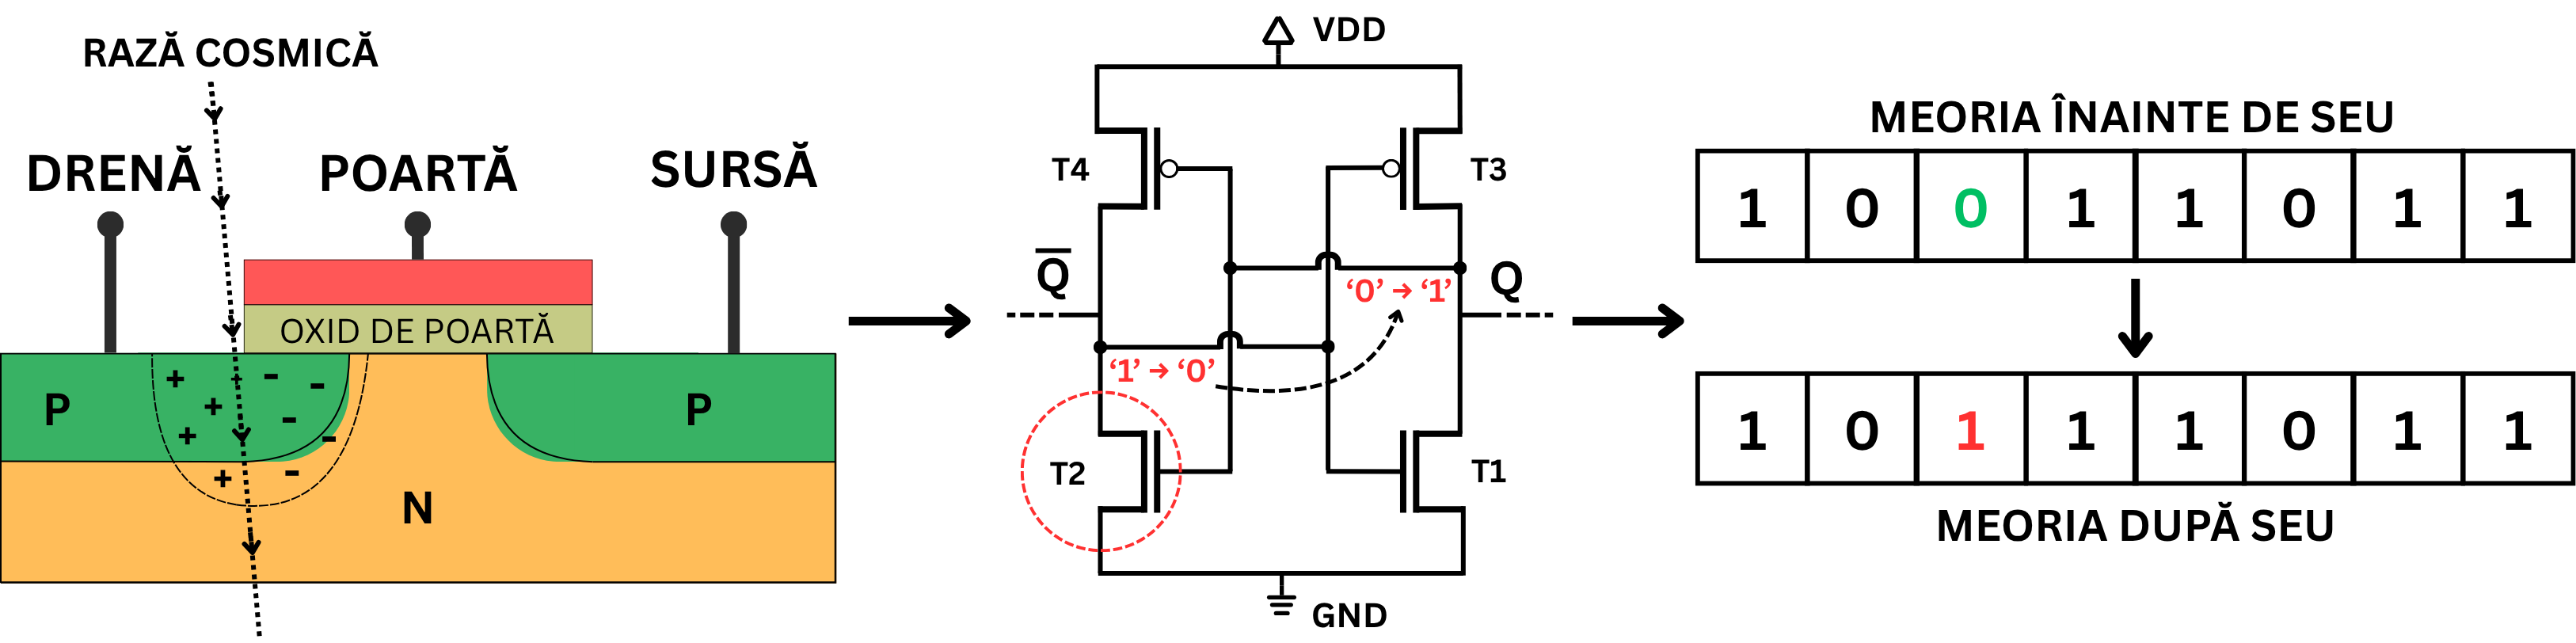
\includegraphics[width=\columnwidth]{./Images/theory_seu_illustration.png}
    \caption{Exemplificarea unui SEU care cauzează un bit-flip într-o celulă SRAM 6T.}%
\label{fig:theory_seu_illustration}
\end{figure}
\begin{table}[ht!]
  \centering
  \renewcommand{\arraystretch}{1.6}
  \caption{Analiză comparativă a unor FPGA-uri similare.}%
  \label{tab:sw_fpga_comparison}
  \begin{tabular}{l c c c c c c c r}
    \toprule
    \textbf{Familie} & \textbf{Nume} & \textbf{FF} & \textbf{LUT} & \textbf{DSP} & \textbf{URAM} & \textbf{BRAM} & \textbf{BRAM [Kb]} & \textbf{Preț} \\
    \midrule
    Artix-7 & XC7A100T & 126.800 & 63.400 & 240 & --- & 135 & 4.860 & \$258 \\
    Artix-7 & XC7A200T & 269.200 & 134.600 & 740 & --- & 365 & 13.140 & \$370 \\
    \midrule
    Artix US+ & AU20P & 218.000 & 109.000 & 900 & --- & 200 & 7.200 & \$587 \\
    Artix US+ & AU25P & 282.000 & 141.000 & 1200 & --- & 300 & 10.800 & \$700 \\
    \midrule
    Kintex US+ & KU3P & 325.440 & 162.720 & 1368 & 48 & 360 & 12.960 & \$2252 \\
    Kintex US+ & KU5P & 433.920 & 216.960 & 1824 & 64 & 480 & 17.280 & \$3056 \\
    \bottomrule
  \end{tabular}
\end{table}
\begin{figure}[h]
    \centering
    \begin{tikzpicture}
        \begin{groupplot}[
            ybar,
            /pgf/bar width=16pt,
            enlarge x limits=0.22,
            enlarge y limits=0.3,
            ylabel={Putere [mW]},
            symbolic x coords={100 MHz, 50 MHz, 10 MHz},
            xtick=data,
            width=8.5cm,
            height=7cm,
            grid=major,nodes near coords,
            tick label style={font=\footnotesize},
            every node near coord/.append style={font=\footnotesize},
            legend style={at={(1.1,-0.2)}, anchor=north, legend columns=3, column sep=7pt},
            group style={group size=2 by 1,horizontal sep=1cm,ylabels at=edge left,vertical sep=0pt}
        ]
        
        % First plot
        \nextgroupplot[title={Consum static}]
        \addplot+[blue, fill=blue!20] coordinates {(100 MHz,  103)(50 MHz,  103)(10 MHz, 102)};
        \addlegendentry{XC7A200T}
        \addplot+[red, fill=red!20] coordinates {(100 MHz,  457)(50 MHz,  455)(10 MHz, 453)};
        \addlegendentry{AU25P}
        \addplot+[brown, fill=brown!20] coordinates {(100 MHz,  457)(50 MHz,  455)(10 MHz, 453)};
        \addlegendentry{KU5P}
        
        % Second plot
        \nextgroupplot[title={Consum dinamic}]
        \addplot+[blue, fill=blue!20] coordinates {(100 MHz,  626)(50 MHz,  366)(10 MHz, 159)};
        \addplot+[red, fill=red!20] coordinates {(100 MHz,  473)(50 MHz,  291)(10 MHz, 140)};
        \addplot+[brown, fill=brown!20] coordinates {(100 MHz,  475)(50 MHz,  290)(10 MHz, 140)};
        
        \end{groupplot}
    \end{tikzpicture}
    \caption{Consumul de energie pentru FPGA-urile din cele trei familii.}%
\label{fig:fpga_power_estimations}
\end{figure}


% ------- BIBLIOGRAPHY IS AUTOMATED - NO NEED TO MODIFY
\printbibliography

\chapter*{Rezumat}
\addcontentsline{toc}{chapter}{Rezumat}

Rezumatul reprezintă o scurtă prezentare a conținutului lucrării de licență, evidențiind obiectivele, metodologia, rezultatele principale și concluziile. Este esențial ca rezumatul să fie concis și clar, oferind cititorului o imagine rapidă asupra temei și contribuțiilor lucrării.

\chapter*{Abstract}
\addcontentsline{toc}{chapter}{Abstract}

The abstract provides a brief summary of the bachelor's thesis, highlighting the objectives, methodology, main results, and conclusions. It is essential for the abstract to be concise and clear, giving the reader a quick overview of the topic and contributions of the work.

% ------- THESE DOCUMENTS ARE MADE SEPARATELY AND ADDED HERE
% ------- NO NEED TO MODIFY HERE - JUST UNCOMMENT
% \newpage
% \addcontentsline{toc}{chapter}{Anexa 1}
% \includepdf[pages=-, pagecommand={\thispagestyle{plainfooter}}]
% {Anexe/Anexa 1.pdf}

% \newpage
% \addcontentsline{toc}{chapter}{Anexa 2} 
% \includepdf[pages=-, pagecommand={\thispagestyle{plainfooter}}]
% {Anexe/Anexa 2.pdf}

% \newpage
% \addcontentsline{toc}{chapter}{Anexa 3}
% \includepdf[pages=-, pagecommand={\thispagestyle{plainfooter}}]
% {Anexe/Anexa 3.pdf}

% \newpage
% \addcontentsline{toc}{chapter}{Declarație privind originalitatea}
% \includepdf[pages=-, pagecommand={\thispagestyle{plainfooter}}]
% {Anexe/Declaratie originalitate.pdf}

\end{document}
